\documentclass[11pt,fancychapters]{article}
\usepackage[a4paper, total={6in, 8in}]{geometry}
\usepackage{cite}
\usepackage{color}
\usepackage{xcolor}
\usepackage{empheq}
\usepackage{enumitem}
\usepackage{setspace}
\usepackage{hyperref}
\usepackage{minted}
\usepackage{acro}
\usepackage{amsmath}
\usepackage{amsthm}
\usepackage{amssymb}
\usepackage{multirow}
\usepackage{graphicx}
\usepackage{geometry}
\usepackage{subcaption}
\usepackage{cancel}
\usepackage[utf8]{inputenc}
\usepackage[english]{babel}
\usepackage{tcolorbox}
\usepackage{hyperref}
\usepackage{cleveref}
\usepackage{parskip}
\usepackage{tcolorbox}
\usepackage{float}
\usepackage{bm}
\usepackage{mathtools}
\usepackage{pgfplots}
 \geometry{
 a4paper,
 total={170mm,257mm},
 left=20mm,
 top=20mm,
 }
\pgfplotsset{width=8cm,compat=1.9}
\newcommand{\dbar}{{d\mkern-7mu\mathchar'26\mkern-2mu}}
\newcommand{\boxedeq}[2]{\begin{empheq}[box={\fboxsep=6pt\fbox}]{align}\label{#1}#2\end{empheq}}
\newcommand{\approptoinn}[2]{\mathrel{\vcenter{
  \offinterlineskip\halign{\hfil$##$\cr
    #1\propto\cr\noalign{\kern2pt}#1\sim\cr\noalign{\kern-2pt}}}}}
\newcommand{\appropto}{\mathpalette\approptoinn\relax}
\renewcommand*{\thesection}{\arabic{section}.}
\def\*#1{\mathbf{#1}}
\def\ab{ab}
\usepackage{tikz}
\usetikzlibrary{calc,trees,positioning,arrows,chains,shapes.geometric,%
    decorations.pathreplacing,decorations.pathmorphing,shapes,%
    matrix,shapes.symbols}
\geometry{top=1.3in,bottom=1.3in}

\DeclarePairedDelimiter\abs{\lvert}{\rvert}%
\DeclarePairedDelimiter\norm{\lVert}{\rVert}%

% Swap the definition of \abs* and \norm*, so that \abs
% and \norm resizes the size of the brackets, and the 
% starred version does not.
\makeatletter
\let\oldabs\abs
\def\abs{\@ifstar{\oldabs}{\oldabs*}}
%
\let\oldnorm\norm
\def\norm{\@ifstar{\oldnorm}{\oldnorm*}}
\makeatother

\begin{document}
\centerline{\huge{SUTD 2021 50.007 Midterm Examination}}

\begin{table}[ht]
\centering
\footnotesize
 \begin{tabular}{c c} 
James Raphael Tiovalen & 1004555
 \end{tabular}
\end{table}

\section*{Problem 1: True or False}

\begin{enumerate}[label=\textbf{\arabic*.}]
	\item True. A training set S can have different geometric margins depending on how the hyperplane is defined. The optimal hyperplane for a given S is the one that gives maximum geometric margin over all possible hyperplanes.
	\item True. A complex learning model can reduce the training error as well as the test error.
	\item True. In clustering, the choice of which distance metric to use is important as it will determine the type of clusters you will find.
	\item True. To use stochastic gradient descent algorithm for minimization, you must have a convex function. Otherwise, it will never let us reach the global optimal value.
	\item True. For a small set of training examples, your model trained on that data will have high variance.
	\item True. In k-medoids clustering algorithm, we can use different distance measures other than the squared Euclidean distance.
	\item True. The hinge loss function allows us to obtain the minimum empirical risk for classification even when the training examples are not linearly separable.
\end{enumerate}

\section*{Problem 2: Multiple Choice Questions}

\begin{enumerate}[label=\textbf{\arabic*.}]
	\item The following statements are true:
	\begin{itemize}[label={-}]
		\item Logistic Regression is a model that is used for classification, not for regression.
		\item Suppose that you have trained a logistic regression classifier, and it outputs on a new example a prediction of 0.67. This means that our estimate for $P(y = 0|x; \theta)$ is 0.33.
	\end{itemize}

	\item Even after we have found a good value for the regularization term $\lambda$ using cross-validation, since we have acquired more data/a larger dataset (more training examples), the $\lambda$ value would need to be decreased.
	
	\item Only the following statement is true:
	\begin{itemize}[label={-}]
		\item The radial basis function kernel is special in many ways. For example, running the SVM with such a kernel function will always be able to return you a separable solution provided the training examples are all distinct.
	\end{itemize}

	\item In SVM, maximum margin linear separators can be found by solving the primal quadratic programming problem:
	
	\begin{equation*}
		\text{min} \enspace \frac{1}{2} \norm{w}^2 \enspace \text{subject to} \enspace d_i(w^Tx_i + b) \geq 1
	\end{equation*}

	\item The problems that can be solved using the K-medoids algorithm include:
	\begin{itemize}[label={-}]
		\item Classification of dogs and cats.
		\item Categorizing news articles into sports, technology, finance and politics categories.
	\end{itemize}

	\item When the $\mathcal{H}$ set is too large (no constraints), the classifier will $\textbf{overfit}$ on the training data and when the $\mathcal{H}$ set is too small, it will $\textbf{underfit}$ the training data.
\end{enumerate}

\section*{Problem 3: Classification}

\begin{enumerate}[label=\textbf{(\alph*)}]
	
\item We can plot a visual, graphical representation of the given data points, as well as one possible classifier:

\begin{figure}[!h]
	\centering
	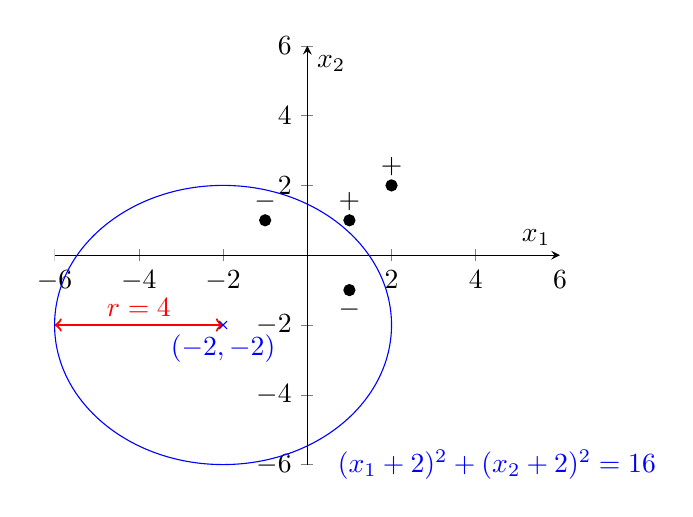
\begin{tikzpicture}
		\begin{axis}[
			axis lines=middle,
			xmin=-6, xmax=6,
			ymin=-6, ymax=6,
			clip=false,
			xlabel=$x_1$, ylabel=$x_2$,
			]
			\addplot [only marks, mark=*, nodes near coords={$+$}] table {
				1 1
				2 2
			};
			\addplot [only marks, mark=*, nodes near coords={$-$}] table {
				-1 1
				1 -1
			};
			\addplot [only marks, mark=x, color=blue, nodes near coords={$(-2,-2)$}] table {
				-2 -2
			};
			\addplot [<->, red, thick] coordinates {(-2,-2) (-6,-2)}
			node at (axis cs:-4,-1.5) {$r = 4$};
			\draw [blue, radius=4] (axis cs:-2,-2) circle
			node at (axis cs:4.5,-6) {$(x_1+2)^2 + (x_2+2)^2 = 16$};
		\end{axis}
	\end{tikzpicture}
\end{figure}

The classifier specified in the diagram has the parameters $a = -2, b = -2, r = 4$. More formally, such a classifier can be defined as

\begin{equation*}
	h(x) = \begin{cases}
		+1, \quad &\text{if} \, ~ (x_1+2)^2 + (x_2+2)^2 \geq 16; \\
		-1, \quad &\text{if} \, ~ (x_1+2)^2 + (x_2+2)^2 < 16 \\
	\end{cases}
\end{equation*}

\item When a training data point $x^{(t)}$ is misclassified, the sign of $(\theta^{(k)} \cdot x^{(t)})$ would disagree with $y^{(t)}$; thus, the product $y^{(t)} (\theta^{(k)} \cdot x^{(t)})$ is non-positive. Given that the updated parameters are given by $\theta^{(k+1)} = \theta^{(k)} + y^{(t)}x^{(t)}$, then when we consider classifying the sample training example $x^{(t)}$ after the update, using the new parameters $\theta^{(k+1)}$, then we would obtain:

\begin{equation*}
	\begin{split}
		y^{(t)} (\theta^{(k+1)} \cdot x^{(t)}) & = y^{(t)} (\theta^{(k)} + y^{(t)}x^{(t)}) \cdot x^{(t)} \\
		& = y^{(t)} (\theta^{(k)} \cdot x^{(t)}) + (y^{(t)})^2 (x^{(t)} \cdot x^{(t)}) \\
		& = y^{(t)} (\theta^{(k)} \cdot x^{(t)}) + \norm{x^{(t)}}^2
	\end{split}
\end{equation*}

Since $\norm{x^{(t)}}^2 > 0$, the value of $y^{(t)} (\theta \cdot x^{(t)})$ is guaranteed to increase as a result of the update (i.e., becomes more positive). As we consider the same training example repeatedly, we will necessarily change the parameters such that the example will be eventually classified correctly (i.e., the value of $y^{(t)} (\theta \cdot x^{(t)})$ becomes positive).

\end{enumerate}

\section*{Problem 4: Regression}

Let the features $x_1, x_2, x_3, x_4$ be the production price, selling price, retail price of competitors, and total number of candies in the market, respectively.

\begin{enumerate}[label=\textbf{\arabic*.}]
	\item For linear regression, we simply want to find the real values of the weights $\theta = \begin{bmatrix}\theta_1 & \theta_2 & \theta_3 & \theta_4\end{bmatrix}^T$ and $\theta_0$ that minimizes the least square loss and optimizes the linear model $f(x;\theta,\theta_0) = \theta_1x_1 + \theta_2x_2 + \theta_3x_3 + \theta_4x_4 + \theta_0$. A possible drawback might be that this model is sensitive to outliers, and we need to assume that each feature is independent from each other, which might not be the case in real life. The model might also be more susceptible to over-fitting. However, this model has a lower computational time complexity.
	
	\item For polynomial regression, we want to find the real values of the weights $\theta$, $\theta_0$, and $N$ that minimizes the least square loss and optimizes a polynomial model of $f(x;\theta,\theta_0)$. This polynomial model will include all powers of each feature up to $N$ (e.g., $x_1^2$, $x_2^2$, etc.), which is the maximum power that we will consider, as well as feature interactions between each feature (e.g., $x_1x_2$, $x_2x_3$, etc.). While a polynomial regression might provide a much better approximation of the relationship between the features and the amount of candy that they will be able to sell, a possible drawback might be that this model is also sensitive to outliers, and it might have a much higher computational time complexity.
	
	\item For ridge regression, our prediction process is similar to the linear regression, except now, we will also add a regularization parameter $\lambda \geq 0$ to the model. This way, we can exclude potentially irrelevant features that might not affect the amount of candy that they will be able to sell at all. However, since the regularization parameter will trade variance for bias, the final estimate using a ridge regression model might be quite biased.
\end{enumerate}

\section*{Problem 5: K-Means}

\begin{enumerate}[label=\textbf{\alph*)}]
	\item For one iteration, we have:
	
	\begin{table}[h!]
		\centering
		\begin{tabular}{|c | c | c | c | c|} 
			\hline
			\multicolumn{2}{|c|}{Data} & \multicolumn{2}{|c|}{Distance to} & Cluster\\
			\cline{1-4}
			$i$ & $z_i$ & $C_1=(1,0)$ & $C_2=(3,2)$ & Assignment\\
			\hline
			1 & (1,0) & 0 & $\sqrt{8}$ & $C_1$ \\ 
			\hline
			2 & (3,2) & $\sqrt{8}$ & 0 & $C_2$ \\
			\hline
			3 & (2,4) & $\sqrt{17}$ & $\sqrt{5}$ & $C_2$ \\
			\hline
			4 & (8,7) & $\sqrt{98}$ & $\sqrt{50}$ & $C_2$ \\
			\hline
			5 & (9,11) & $\sqrt{185}$ & $\sqrt{117}$ & $C_2$ \\
			\hline
			6 & (10,10) & $\sqrt{181}$ & $\sqrt{113}$ & $C_2$ \\ [1ex] 
			\hline
		\end{tabular}
	\end{table}

	\item We need at least $\textbf{two}$ iterations to converge to the final cluster assignments ($\textbf{three}$, if we include the additional final check, at which there will be no more changes to the cluster assignments). The final cluster assignments would be: $C_1 = \{z_1, z_2, z_3\}$ and $C_2 = \{z_4, z_5, z_6\}$.
	
	\item Euclidean distance of $z_7$ to $C_1$ is $\sqrt{(11-2)^2 + (8-2)^2} = \sqrt{117}$, while Euclidean distance of $z_7$ to $C_2$ is $\sqrt{(11-9)^2 + (\frac{28}{3}-8)^2} = \sqrt{\frac{52}{9}}$. Hence, since $\sqrt{\frac{52}{9}} < \sqrt{117}$, $z_7$ will be assigned to cluster $C_2$.
\end{enumerate}

\section*{Problem 6: SVM}

\begin{enumerate}[label=\textbf{\arabic*.}]
	\item This is because from one of the KKT conditions, we have $C = \alpha_i + \beta_i$. Since $\alpha_i = C - \beta_i$, $\alpha_i \ge 0$, and $\beta_i \ge 0$, we can combine said constraints to form the constraint $0 \le \alpha_i \le C$.
	
	\item The kernel trick is to find $K(x, x') = \varphi(x)\varphi(x') = \text{exp}(-\frac{\norm{x-x'}}{2})$ instead of finding the explicit form of $\varphi(x)$ or $\varphi(x')$, which is much more difficult. It is useful when the data is not linearly separable, and when we want to transform the data into a higher dimension space to make it linearly separable. For example, by using a radial basis function kernel, we can run SVM and always obtain a separable solution (provided that the training examples are distinct).
	
	\item Yes. A polynomial with degree 0 is a valid kernel, since it is symmetric and positive semi-definite.
	
	\item Yes, since it is symmetric and positive semi-definite.
	
	\item No, since while it is symmetric, it is not positive semi-definite (due to the $-8$).
	
	\item No, since it is not symmetric.

\end{enumerate}

\section*{Problem 7: Logistic Regression}

\begin{enumerate}[label=\textbf{(\alph*)}]
	
	\item We might need logistic regression when we need to classify whether a tumor is malignant or benign. The data will be labelled. The input will be labelled tumor images, while the outputs will be the probability that it is malignant. We might prefer using logistic regression over SVM since the data might not be linearly separable, and that we want to know the probability of the tumor being malignant.
	
	\item Given that $\theta = \begin{bmatrix}-1 & 0 & 0 & 4 & 9\end{bmatrix}^T$, we have:
	
	\begin{equation*}
		y = \begin{cases}
			1, \quad &\text{if} \, ~ -1 + 4x_1^2 + 9x_2^2 \geq 0; \\
			0, \quad &\text{if} \, ~ -1 + 4x_1^2 + 9x_2^2 < 0 \\
		\end{cases}	
	\end{equation*}
	
	We can rearrange the inequalities to obtain our decision boundary as:
	
	\begin{equation*}
		y = \begin{cases}
			1, \quad &\text{if} \, ~ 4x_1^2 + 9x_2^2 \geq 1; \\
			0, \quad &\text{if} \, ~ 4x_1^2 + 9x_2^2 < 1 \\
		\end{cases}	
	\end{equation*}
	
	Graphically, we can visualize the decision boundary as an ellipse centered at $(0, 0)$, with major axis of length $1$ and minor axis of length $\frac{2}{3}$. We can plot the diagram as such:
	
	\begin{figure}[!h]
		\centering
		\begin{tikzpicture}
			\begin{axis}[
				axis lines=middle,
				xmin=-1, xmax=1,
				ymin=-1, ymax=1,
				clip=false,
				xlabel=$x_1$, ylabel=$x_2$,
				]
				\addplot[domain=0:360,data cs=polar, samples=200,
				line width=0.7pt, green] (x,{1/(3*(sqrt(1-(5*cos(x)*cos(x))/9)))});
			\end{axis}
		\end{tikzpicture}
	\end{figure}

	\pagebreak
	
	\item No, it will not change. This is because the new data will be test data, instead of being considered as training data.
	
\end{enumerate}

\section*{Problem 8: Neural Networks}

Output of $h_1$ is 0 since $g(x) = (-1) \cdot 2 + 2 \cdot 1 + (-1) \cdot 2 = -2 + 2 - 2 = -2 < 0$, while output of $h_2$ is 1 since $g(x) = 0 \cdot 2 + (-1) \cdot 1 + 1 \cdot 2 = 0 - 1 + 2 = 1 \geq 0$. Hence, final output is $2$, since $g(x) = 0 \cdot 1 + 1 \cdot 2 = 0 + 2 = 2 \geq 0$.

\end{document}
